\tikzstyle{env} = [rectangle, rounded corners, text centered, draw=black, fill=red!30]
\tikzstyle{vert} = [rectangle, rounded corners, minimum width=3cm, minimum height=1cm, text centered, draw=black, fill=blue!30]

\section{Overview}
The communications module class, \textit{CommMod}, is the part of the simulator solution that is responsible for performing tasks at level three of the OSI model (the networking layer). Depending on the noise function used by the simulator, it is also possible to have communications modules perform tasks in layer two (such as collision detection and avoidance). Whilst the base class is a part of the simulator itself, the actual implementation of routing algorithms are part of a separate library in their own right. In this way, the communications library is intended to be distributed with \textbf{octoDrone} without being a required constituent part.

\section{Structure}
\subsection{Structure of an Individual Module}
\subsubsection{Sending and Receiving Messages}
		
When a communications module wishes to transmit a message to other units it invokes the broadcast method exposed by the simulation environment. Messages that originate from the communication modules messageable collect in a queue, which must be checked at regular intervals. When there is a message that the environment determines should be delivered to the communications module, it is deposited in a similar queue. When the module has a message it needs to pass to its messageable, it stores it in a third queue.

In addition to asynchronous messaging, the project design also called for synchronous message passing. This is achieved by having a callback function in the messagable which can be invoked upon receipt of an urgent communication. It is left to the communication implementation to decide which messages are important to interrupt the normal operation of the messageable for.
		
\subsubsection{Intermediate Processing}
The virtual function \textit{comm\_function} is called when the communications module is started and is expected to return when the associated program is ready to terminate. It should be used to perform any intermediate and non-delivery driven processing such as routing or time based commands.
		
\subsection{Structure of a Collection of Modules}
	
In order to facilitate easy distribution and use, collections of communication implementations are combined into libraries. Given the small size of a communications modules source code (often tens of kilobytes) it might be tempting to statically link them to simulation executables. The problem with this approach, however, is that it precludes the very thing that prompted the creation of communications modules in the first place - modularity. As such, communications code is packaged into a shared library which simulator executables are then linked against dynamically at compile time. This reduces the size of produced executables and makes updating communications code possible without requiring simulations to be recompiled.

\subsection{Access to Other Simulation Elements}
		
The architecture of the simulator requires that communications modules are able to interact with the simulator environment (to dispatch messages), as well as with the messageable with which they are associated. Since it is impossible to have all of this information available when the communications module is instantiated (creating a messageable requires a reference to a communications module as well), it is necessary to set the messageable associated with a communications object at a later time (but before the simulation is started). Thus, the procedure for bootstrapping a simulation is broadly as follows:

\begin{enumerate}
	\item Load the sensor data
	\item Create a simulation environment referencing the sensor data
	\item Create a communications module referencing the environment
	\item Create a messageable referencing the environment and the communications module
	\item Add a reference to the messageable to the communications module
\end{enumerate}

How these references are used is covered in section \ref{int-sim}.

\section{Integration with the Simulator and other Programs}
\label{int-sim}
The communications module class makes use of the following functions from the simulator:

\begin{itemize}
\item \textit{broadcast}
\end{itemize}

Programs for drones and base stations can make use of the following functions from \textit{CommMod}:

\begin{itemize}
\item \textit{push\_in\_message}
\item \textit{push\_out\_message}
\item \textit{comm\_function} (to start the CommMod)
\item \textit{set\_messageable} (used when defining simulations)
\end{itemize}

\section{Provided Implementations}
\begin{figure}[H]
\centering
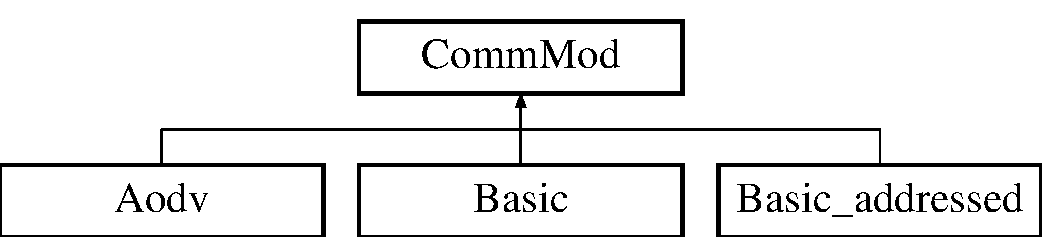
\includegraphics[scale=0.4]{../documentation/latex/class_comm_mod}	
\caption{Inheritance diagram for the \textit{CommMod} class}
\end{figure}

\subsection{Basic Messaging}
\begin{figure}[H]
\centering
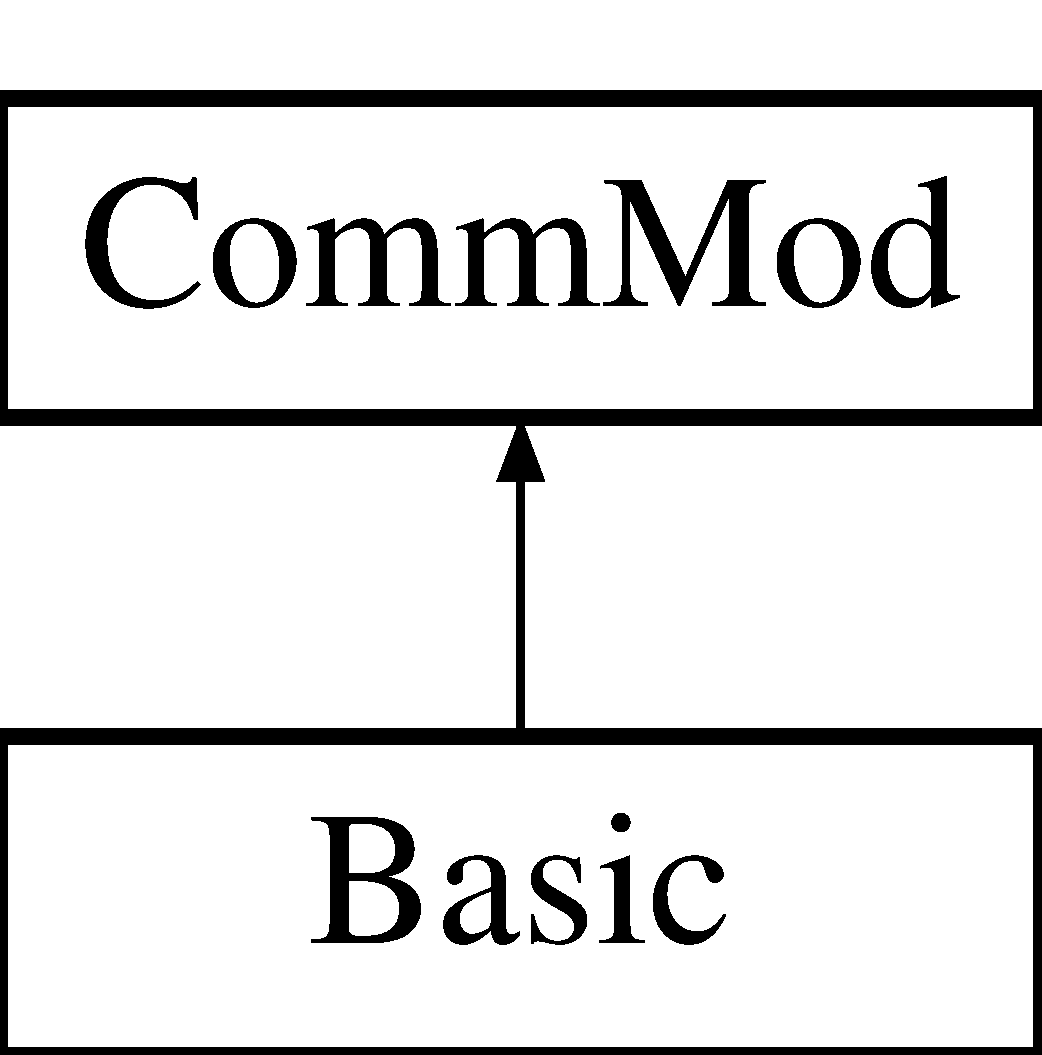
\includegraphics[scale=0.2]{../documentation/latex/class_basic}	
\caption{Inheritance diagram for the \textit{Basic} class}
\end{figure}

The basic messaging implementation provides the simplest possible way of sending and receiving messages. This can be useful when creating programs for messageable units, as it removes the need to consider routing problems, units being out of range, and a whole host of other potential issues. Additionally, it provides a good method for simulating existing programs which were not written with \textbf{octoDrone} in mind and may perform their own addressing. In this way it contributes to octoDrones ability to be generic and flexible. 

In this implementation, all messages that are sent are received by all nodes, regardless of range. Messages sent include payload information, but do not store information on the sender or receiver.
	
\subsection{Addressed Basic Messaging}
\begin{figure}[H]
\centering
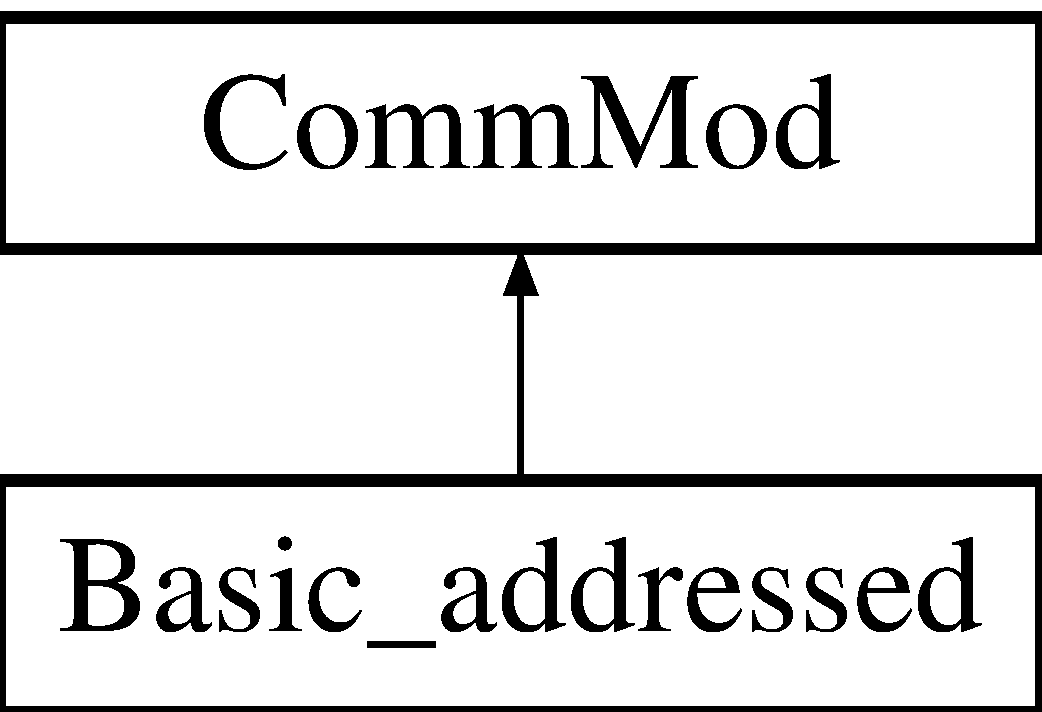
\includegraphics[scale=0.2]{../documentation/latex/class_basic__addressed}
\caption{Inheritance diagram for the \textit{Basic\_addressed} class}
\end{figure}

The addressed basic messaging implementation extends the above algorithm to additionally take into account the sender and intended recipient of a message when choosing which packets to deliver and which to drop. It is intended to be used for passing messages between programs and communication modules in a way which prevents the need to include code to serialise and deserialise addresses. If appropriate, it can also be used with external programs as described above.

In this implementation, all messages that are sent to an IP address are received by all nodes with that IP address, regardless of range. Messages include payload information as well as the IP addresses of the sender and intended recipient. Messages sent to the broadcast address 255.255.255.0 will be received by all nodes in the simulation.	
	
\subsection{Ad hoc On-Demand Distance Vector Routing}
\begin{figure}[H]
\centering	
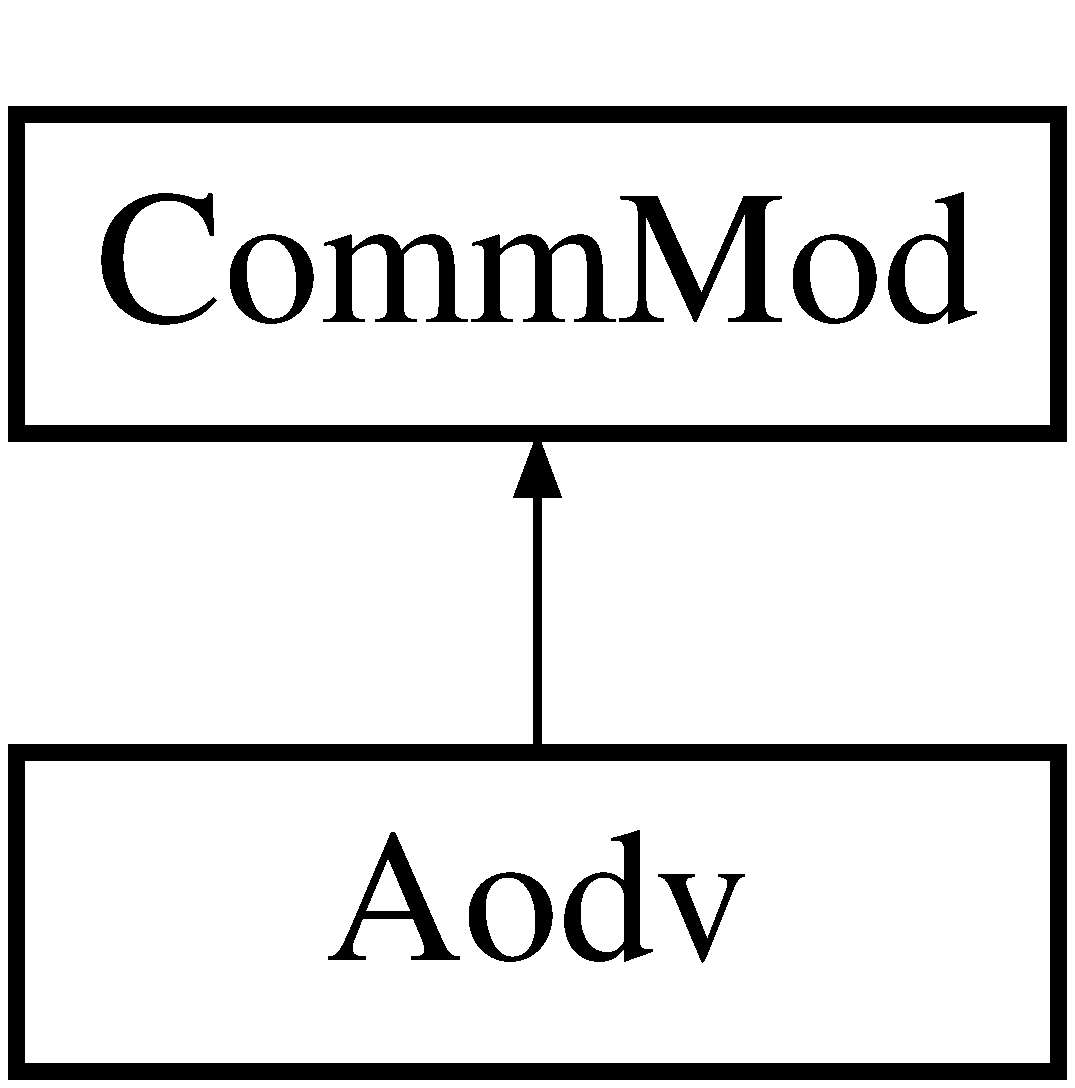
\includegraphics[scale=0.2]{../documentation/latex/class_aodv}	
\caption{Inheritance diagram for the \textit{Aodv} class}
\end{figure}

The Ad hoc On-Demand Distance Vector Routing (AODV) implementation provided in the communications library gives an example of how a more sophisticated routing algorithm can be used within the simulator framework. AODV is designed to be used in mobile ad hoc networks and offers loop free, just-in-time routing that is fault tolerant and capable of reacting to the movement of nodes.

\subsubsection{Overview}
In order to explain what is happening under the hood of the AODV implementation provided with \textbf{octoDrone} it will be useful to first cover the basics of how the algorithm operates\cite{perkins2003}. A node A which wishes to send a data packet to node Z transmits a Route Request (RREQ) to its neighbours, which serves the dual purpose of notifying it of the next hop in the most efficient path to Z, but also of notifying the routes along the way where they should direct messages addressed to Z. If a unit receives a route request for which it does not have a valid route it broadcasts the route request to each of its neighbours in order to propagate the route discovery. 

When the RREQ is received by a node which has a route to Z, either because (as in this case) it \textit{is} node Z or because it is already part of a route to Z, that node creates and returns a Route Reply (RREP) packet. This packet is used by every node on the reverse route to store the next hop to the destination, Z, and is forwarded to the nodes that sent the RREQ. Incremented sequence numbers are used to make sure that information remains fresh as for loop prevention. 

Once the sending node, A, receives an RREP it can send out its data packets via the next hop on the route that was just discovered. This route will be cached for a period of time before a new discovery period must take place. If at any time there is an error during transmission, the node encountering the issue sends out a Route Error (RERR) packet to notify other nodes that cached routes using this hop should be invalidated.

\subsubsection{The Routing Table}
The AODV implementation has a special data structure to represent entries in an AODV routing table. As per the RFC (documents by the Internet Engineering Task Force containing technical and organizational notes about topics such as internet protocols), this contains the sequence number of the destination node, the time after which the route is no longer considered active, the hop count to the destination node, and the next hop on the route to the destination node. Each AODV communications module keeps a map of destination IP addresses to route objects, which is known as its routing table.

\subsubsection{Message Types}
\begin{figure}[H]
\centering	
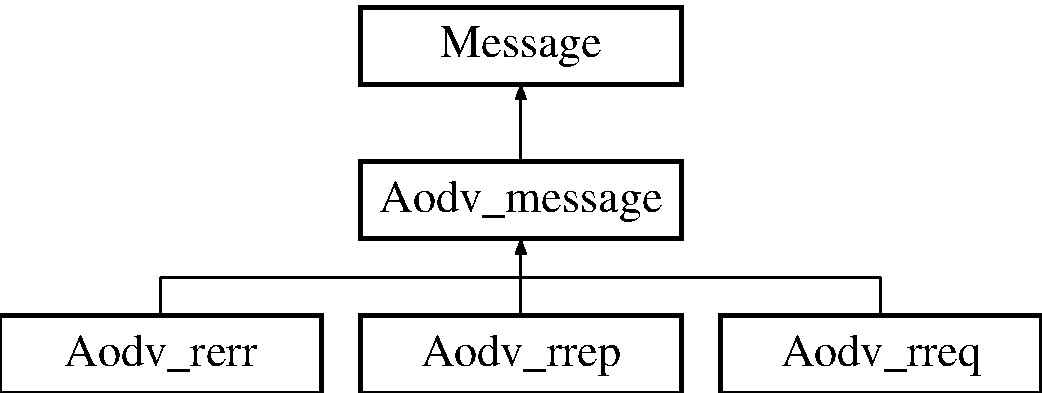
\includegraphics[scale=0.4]{../documentation/latex/class_aodv__message}	
\caption{Inheritance diagram for the \textit{Aodv\_message} class}
\label{aodvmess}
\end{figure}

In order to easily handle the different types of messages handled by AODV (RREQ, RREP, etc.), the implementation defines a basic AODV specific message class which contains the fields common to all AODV messages. This is then extended by individual classes in order to completely define which fields are required by each message type. This is shown in figure \ref{aodvmess}.

\subsubsection{Sending Messages}
With the above classes in mind, we turn to the question of how octoDrone goes about sending messages. Initially, messages which have been deposited into the outbound queue must be deserialised into a structure containing the message payload, the destination address of the message, and the source address of the message (in some situations this may be different from the address of the communications module). This happens because messages are always sent to and received from the environment in string form. While it may at first seem inconvenient, it is necessary in order to preserve the integrity of messages if they are sent over a network (which is the case if we are running a deployment on real hardware). After this the routing table is queried to find out if the node already has an active route to the destination. If it does, then a data packet is constructed immediately and dispatched via the next hop on the route to the destination.

If there does not exist a route in the cache, things become a little more complicated. Because the route discovery process requires that we send and receive a number of different packets before sending the message is considered done, we need to keep track of internal state. In octoDrone's implementation of AODV, this is done by keeping track of the current message we are sending, as well as the stage in the route discovery process we are currently at. This means that whenever something is triggered by a message being received, it can access this information (and update it if required), even when the original message object has long since gone out of scope. After the state information is created, a helper function is used to create the RREQ which will initiate the AODV protocol on other nodes. This is then sent using a call to the simulation environment. At this point there is nothing else to do but wait for messages to be received.

\subsubsection{Receiving Messages}
When a message is received, the communications module unwraps just enough of it to determine the type of message that has been delivered, which will be one of the AODV types, such as RREQ (this type is internal to AODV, and should not be confused with the type property of the base message class which is used to denote emergency packets). This information is then used to select an appropriate deserialisation function to apply to the message in order to transform it from a string into an AODV data type. Each of the types has its own processing method, which determines what action (if any) to take given the message contents and the internal state of the communications module.

For RREQ messages, the node checks to see if the message was a hello message (described in section \ref{hello}), and if so we determines if there is an active route to the sender (who will be one of its neighbours), and add a new route if it does not. A reply is sent to the sending node so that it can compile route information about other units in the network. If it is not the case that the message is a hello message, then it must be route discovery from another node. If the communications module has an active route to the destination mentioned in the RREQ, then a helper method is used to generate an RREQ packet to reply with. This is sent via a call to the simulation environment. Otherwise, the node's internal state is updated to record that it is participating in remote initiated route discovery, and the RREQ packet is forwarded after decrementing the time to live (TTL) field and incrementing the hop count. In order to keep the implementation small and simple, nodes do not respond to RREQ requests when they are part way through route discovery for themselves or another node.

When an RREP is received, the communication module first checks to see if the route it has to the sender (previous hop) is up to date, modifying the routing table if appropriate. Afterwards, it checks to see if the route was for itself (to send a data packet) or for another node (remote initiated route discovery). Multiple RREP packets for a single route indicate that there exists more than one possible path. In this case, the route with the lowest hop count is chosen (the reply window is defined by the path discovery time variable which is set at instantiation). If the former, then a data packet is constructed using the new routing information, and sent via a call to the simulation environment. Otherwise, the information is passed on (with a decremented TTL). Keeping track of hop counts is done by the helper function.

Upon receipt of an RERR packet, the communication module marks the route as invalid (achieved here by setting the active route timeout to zero), before broadcasting this information so that affected nodes can update their local routing tables.

\subsubsection{Broken Links}
But where do these RERR packets come from? It may be that a node receives a message for which it does not have a route. It may also occur that a node loses connectivity with one of its neighbours. If either of these scenarios come to pass then the receiving node will broadcast an RERR message to the node which precedes it in the route. Given that the octoDrone implementation of AODV only stores forward routes for simplicity, all RERR messages are sent upon message receipt instead of also being sent upon link failure. This makes sense: because octoDrone does not emulate the lower layers of the OSI model, nodes do not have access to information about link statuses. One way of mitigating this is to use hello packets as described below in section \ref{hello}. When a node fails to receive a hello packet for a neighbour which is listed as the next hop for one of the route in its routing table (this includes neighbours which are the next hop and destination for a route), it will mark that route as invalid and propagate an RERR the next time that route is used.

\subsection{Extension: Hello Messages}
\label{hello}
The RFC for AODV also mentions the use of hello messages as a means of broadcasting connectivity information. While the document suggests that nodes should only broadcast hello messages if they are part of an active route, to account for the differences mentioned above, all nodes using the octoDrone implementation of AODV will send hello packets on a regular basis.

\section{Summary}
The above sections have shown how the designs for octoDrone communications have been implemented, covering the structure of communication modules, message types, and how these components integraye with the rest of the software. In the next chapter these concepts will be taken one step further with the jump to real hardware instead of simulated hardware as was discussed here.